\documentclass[aspectratio=169,11pt]{beamer}

% ================================================================
% "TABIIY TILNI QAYTA ISHLASH" KURSI
% MA'RUZA 2 --- Klassik usullar bilan matnlarni tasniflash,
%               klassifikator modellarni baholash va NLPdagi etika
%              (d02_klassik_tasnif.tex)
% Arxetiplar: [A][B][C][D][E] + 4 tsikl [F][G][H][I][J][K][L] +
%             [M][N][O][P][Q][R] + ilova [S]
% Rendered slayd soni: ~49  (grafikli versiya)
% ================================================================

% ================================================================
% RANGLAR  (asl fayldan o'zgarishsiz)
% ================================================================
\definecolor{cnublue}{rgb}{0.07,0.14,0.62}
\definecolor{cnubluelight}{rgb}{0.18,0.30,0.72}
\definecolor{cnubluebg}{rgb}{0.90,0.92,0.97}
\definecolor{deepblue}{rgb}{0.07,0.14,0.62}
\definecolor{deepred}{rgb}{0.60,0.00,0.00}
\definecolor{deepgreen}{rgb}{0.00,0.45,0.00}
\definecolor{halfgray}{gray}{0.55}

% ================================================================
% BEAMER MAVZU --- Boadilla + maxsus footer  (asl fayldan o'zgarishsiz)
% ================================================================
\usetheme{Boadilla}

\setbeamercolor{structure}{fg=cnublue}
\setbeamercolor{frametitle}{bg=cnublue,fg=white}
\setbeamercolor{title}{bg=cnublue,fg=white}
\setbeamercolor{block title}{bg=cnublue,fg=white}
\setbeamercolor{block body}{bg=cnubluebg,fg=black}
\setbeamercolor{alerted text}{fg=deepred}
\setbeamercolor{author in head/foot}{bg=cnubluelight,fg=white}
\setbeamercolor{section in head/foot}{bg=cnublue,fg=white}
\setbeamercolor{page number in head/foot}{bg=cnubluelight,fg=white}

\setbeamertemplate{mini frame}{}
\setbeamertemplate{mini frame in current section}{}
\setbeamertemplate{mini frame in current subsection}{}
\setbeamertemplate{headline}{}
\setbeamertemplate{navigation symbols}{}

\setbeamertemplate{footline}{%
  \leavevmode%
  \hbox{%
    \begin{beamercolorbox}[wd=0.17\paperwidth,ht=2.5ex,dp=1.25ex,leftskip=0.5em]{author in head/foot}%
      \usebeamerfont{author in head/foot}\scriptsize\insertshortauthor%
    \end{beamercolorbox}%
    \begin{beamercolorbox}[wd=0.69\paperwidth,ht=2.5ex,dp=1.25ex,center]{section in head/foot}%
      \usebeamerfont{section in head/foot}%
      \scriptsize\insertsectionnavigationhorizontal{0.69\paperwidth}{}{}%
    \end{beamercolorbox}%
    \begin{beamercolorbox}[wd=0.14\paperwidth,ht=2.5ex,dp=1.25ex,rightskip=0.5em]{page number in head/foot}%
      \hfill\scriptsize\color{white}%
      \insertframenumber{}/\inserttotalframenumber%
    \end{beamercolorbox}%
  }%
  \vskip0pt%
}

% ================================================================
% PAKETLAR  (asl fayldan o'zgarishsiz)
% ================================================================
\usepackage[utf8]{inputenc}
\usepackage[T1]{fontenc}
\usepackage{lmodern}
\usepackage{amsmath,amssymb}
\usepackage{booktabs}
\usepackage{xcolor}
\usepackage{listings}
\lstset{
    language=Python,
    basicstyle=\ttfamily\tiny,
    keywordstyle=\bfseries\color{deepblue},
    emphstyle=\ttfamily\color{deepred},
    stringstyle=\color{deepgreen},
    commentstyle=\itshape\color{halfgray},
    numbers=none, % kod bloklarida chap numeratsiya ko'rsatilmaydi
    numberstyle=\scriptsize\color{halfgray},
    rulesepcolor=\color{cnublue!30},
    frame=shadowbox,
    xleftmargin=0pt,
    breaklines=true,
    showstringspaces=false,
    tabsize=2
}
\usepackage{tcolorbox}
\tcbuselibrary{skins}
\tcbset{
  defbox/.style={colback=cnubluebg,colframe=cnublue,
                 fonttitle=\small\bfseries\color{white},
                 attach boxed title to top left={yshift=-2mm,xshift=4mm},
                 boxed title style={colback=cnublue,colframe=cnublue}},
  warnbox/.style={colback=orange!8,colframe=orange!70!black,
                  fonttitle=\small\bfseries},
  okbox/.style={colback=green!7,colframe=green!55!black,
                fonttitle=\small\bfseries}
}
\usepackage{tikz}
\usetikzlibrary{arrows.meta,positioning,calc,backgrounds}

% ================================================================
% INTUITIV GRAFIKLAR UCHUN YORDAMCHI USLUBLAR
% (har bir matematik formula yonidagi vizualizatsiyalar uchun)
% ================================================================
\tikzset{
  ax/.style={->,thick},
  curveA/.style={cnublue,very thick,smooth,samples=120},
  curveB/.style={deepred,very thick,smooth,samples=120},
  curveC/.style={deepgreen!65!black,very thick,smooth,samples=120},
  helperln/.style={dashed,thin,halfgray},
  dotB/.style={circle,fill=cnublue,inner sep=1.2pt},
  dotR/.style={circle,fill=deepred!85!black,inner sep=1.2pt},
  dotG/.style={circle,fill=deepgreen!80!black,inner sep=1.2pt},
  tlab/.style={font=\tiny},
}

% ================================================================
% QO'SHIMCHALAR  (asl fayldan o'zgarishsiz)
% ================================================================
\AtBeginSection[]{%
  \begin{frame}{Prezentatsiya rejasi}
    \tableofcontents[currentsection]
  \end{frame}}

\newcommand{\bunda}[1]{{\small\textbf{bunda:}\; #1}}
\newcommand{\bajarildi}{{\color{deepgreen}\large$\checkmark$}\;}

% ================================================================
% METAMA'LUMOT
% ================================================================
\title[Klassik Tasnif]{Klassik usullar bilan matnlarni tasniflash}
\subtitle{Tabiiy tilni qayta ishlash --- 2-ma'ruza}
\author[A.A.\,Abdulali]{A.A.\,Abdulali}
\date{16-iyun 2026}
\institute{11:00--12:20 \quad$\cdot$\quad  mavzu \textnumero{}2}

% ================================================================
\begin{document}
% ================================================================

% ----------------------------------------------------------------
% [A] TITUL
% ----------------------------------------------------------------
\maketitle

% ================================================================
\section[Kirish]{Kirish: vektordan sinfgacha}
% ================================================================

% ----------------------------------------------------------------
% [B] TAKRORLASH: L1 dan ikki savol
% ----------------------------------------------------------------
\begin{frame}{Takrorlash: L1 natijalarini tekshiramiz}
  \begin{columns}[T]
    \begin{column}{0.49\textwidth}
      \begin{tcolorbox}[warnbox,title=Savol 1]
        \small
        $D_1{=}$``nlp qiziq'',\; $D_2{=}$``python foydali'',\;
        $D_3{=}$``nlp foydali''\\[3pt]
        $\mathrm{TF\text{-}IDF}(\text{qiziq},\,D_1) = ?$\\
        \footnotesize [$\mathrm{df}=1$,\; $N=3$,\; $\mathrm{TF}=1$]
      \end{tcolorbox}
    \end{column}
    \begin{column}{0.49\textwidth}
      \begin{tcolorbox}[warnbox,title=Savol 2]
        \small
       BoW vektori $[1,\,1,\,0,\,0]$ nimani \textbf{saqlaydi}?\; Nima \textbf{yo'qoladi}?
      \end{tcolorbox}
    \end{column}
  \end{columns}
  \pause
  \vspace{4pt}
  \begin{columns}[T]
    \begin{column}{0.49\textwidth}
      \begin{tcolorbox}[okbox,title=Javob 1]
        \small
        $\mathrm{IDF}=\ln(3/1)\approx 1.099$\\
        $\mathrm{TF\text{-}IDF}=1\times 1.099=\mathbf{1.099}$
      \end{tcolorbox}
    \end{column}
    \begin{column}{0.49\textwidth}
      \begin{tcolorbox}[okbox,title=Javob 2]
        \small
        Saqlaydi: so'zlar \textbf{chastotasi}.\\
        Yo'qoladi: so'z \textbf{tartibi} (word order).\\
        \footnotesize\textcolor{halfgray}{Bugun: shu vektorlar asosida tasniflash qilamiz.}
      \end{tcolorbox}
    \end{column}
  \end{columns}
\end{frame}

% ----------------------------------------------------------------
% [C] MAQSADLAR
% ----------------------------------------------------------------
\begin{frame}{Bugungi maqsadlar}
  \begin{enumerate}\setlength{\itemsep}{7pt}
    \item \textbf{Keltirib chiqara olasiz:} logistik regressiya gradienti ---
          $\sigma(z)\!\to\!\ell_i\!\to\!L\!\to\!\partial L/\partial w_j$ ---
          uch asosiy bosqichda. 
    \item \textbf{Hisoblay olasiz:} Naive Bayes posterior nisbatini
          Laplace silliqlash (Laplace smoothing) bilan.
    \item \textbf{Qurasiz:} confusion matrix dan accuracy, precision, recall va $F_1$ metrikalarini.
    \item \textbf{Tanqidiy baho bera olasiz:} sentiment klassifikatorida
          kamida uch etika muammosini aniqlaysiz.
  \end{enumerate}
  \vspace{5pt}
  \begin{tcolorbox}[defbox,title=Oldingi bilimlar]
    \small
   Minimum talablar: TF-IDF vektori (L1);\; Python funksiyalar;\;
    $\exp(\cdot)$ va $\ln(\cdot)$ tushunchalari.
  \end{tcolorbox}
\end{frame}

% ----------------------------------------------------------------
% [D] REJA
% ----------------------------------------------------------------
\begin{frame}{Dars rejasi: to'rt blok}
  \begin{center}
    \small
    \begin{tabular}{clr}
      \toprule
      Blok & Mavzu & Vaqt \\
      \midrule
      1 & Logistik regressiya: sigmoid $\to$ gradient & 22 daq \\
      2 & Naive Bayes: Bayes teoremasi + Laplace silliqlash & 25 daq \\
      3 & Metrikalar: confusion matrix, precision, recall, $F_1$ & 20 daq \\
      4 & NLPda etika: uch muammo, oqibatlar & 10 daq \\
      \midrule
        & Xulosa va P2 ko'prigi & 3 daq \\
      \bottomrule
    \end{tabular}
  \end{center}
  \vspace{4pt}
  \small\textcolor{halfgray}{Amaliyotdagi misollar o'zbek matnlari asosida, CPU muhitida ham bajariladigan tarzda beriladi.}
\end{frame}

% ----------------------------------------------------------------
% [E] MUAMMO: TF-IDF vektori bor lekin sinf yo'q
% ----------------------------------------------------------------
\begin{frame}{Bugungi darsda yechiladigan muammo}
  \begin{columns}[T]
    \begin{column}{0.52\textwidth}
      \small
      \textbf{L1 da to'xtagan vaziyatimiz:}\\[4pt]
      Sharh: ``Sifati \textbf{yaxshi}, ammo
      yetkazib berish xizmati sifati \textbf{past} edi.''\\[5pt]
      TF-IDF ning har bir so'z uchun qiymati:\\[2pt]
      \begin{tcolorbox}[warnbox]
        \footnotesize
        yaxshi:\;0.51\quad past:\;0.38\quad
        sifat:\;0.44\quad ammo:\;0.22
      \end{tcolorbox}
      \vspace{5pt}
      \textbf{Sodda qoidaga asoslangan model:} ``yaxshi'' bor $\Rightarrow$ ijobiy sharh?\\
      \alert{Xato!} ``ammo past'' kontentini yetarlicha baholamaydi.
    \end{column}
    \begin{column}{0.44\textwidth}
      \vspace{8pt}
      \begin{tcolorbox}[defbox,title=NLP yondashuvi]
        \small
        TF-IDF vektor $\mathbf{x}$\\[2pt]
        $\downarrow$\\[2pt]
        \textbf{Matematik model}\\[2pt]
        $\downarrow$\\[2pt]
        $P(\text{ijobiy}\mid\mathbf{x})$\\[2pt]
        $\downarrow$\\[2pt]
        Qaror ($>\!0.5$ ?)
      \end{tcolorbox}
      \vspace{5pt}
      \small Bugun ikkita modelni qarab chiqamiz:\\
      \quad 1.\ Logistik regressiya\\
      \quad 2.\ Naive Bayes
    \end{column}
  \end{columns}
\end{frame}

% ================================================================
\section[Log.\ Reg.]{Logistik regressiya}
% ================================================================

% ----------------------------------------------------------------
% [F1] INTUITSIYA: ehtimollikka asoslangan qaror
% ----------------------------------------------------------------
\begin{frame}{Logistik regressiya: nima uchun ehtimollik?}
  \begin{columns}[T]
    \begin{column}{0.50\textwidth}
      \small
       \textbf{Nima uchun ehtimollikka muhtojmiz?}\\[5pt]

      \textbf{``Ikki qiymat'' yetarli emas:}\\[5pt]
      \begin{tabular}{@{}p{4.5cm}l@{}}
        ``Zo'r mahsulot!'' & ijobiy \\[2pt]
        ``Mahsulot yaxshi ammo\ldots'' & noaniq? \\[2pt]
        ``Yomon edi.'' & salbiy \\
      \end{tabular}
      \vspace{6pt}\\
      Model ikkinchi qatordagi
      \textbf{noaniqlikni} ifodalashi kerak.
    \end{column}
    \begin{column}{0.47\textwidth}
      \begin{tcolorbox}[defbox,title=Ehtimollik beradi]
        \small
        $P(\text{ijobiy})=0.95$ --- ishonchli\\[2pt]
        $P(\text{ijobiy})=0.53$ --- noaniq\\[2pt]
        $P(\text{ijobiy})=0.08$ --- salbiy\\[4pt]
        \textbf{Qaror chegarasini turli vazifalarga moslashtirish:}\\
        spam filtri: $>\!0.90$\\
        tibbiy skrining: validatsiya asosida pastroq chegara
      \end{tcolorbox}
    \end{column}
  \end{columns}
\end{frame}

% ----------------------------------------------------------------
% [F1b] RASM: sigmoid egri chiziq (z -> ehtimollik)
% ----------------------------------------------------------------
\begin{frame}{Sigmoid funksiyasi: $z$ ni ehtimollikka aylantiradi}
  \begin{columns}[T]
    \begin{column}{0.54\textwidth}
      \centering
      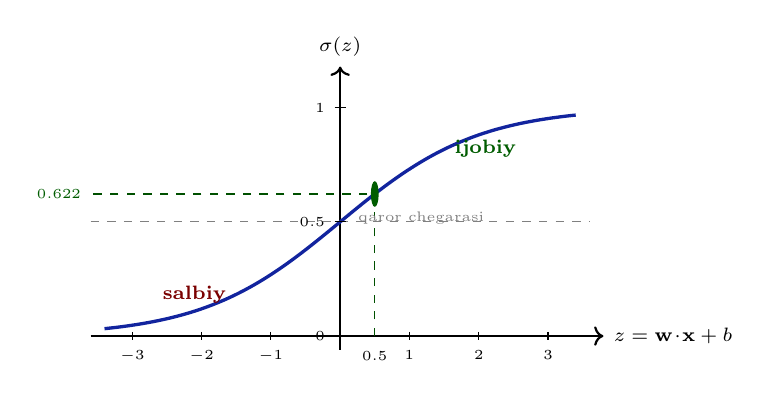
\begin{tikzpicture}[xscale=0.88,yscale=2.9]
        % ---- o'qlar ----
        \draw[->,thick] (-3.6,0)--(3.8,0)
            node[right,font=\scriptsize]{$z=\mathbf{w}\!\cdot\!\mathbf{x}+b$};
        \draw[->,thick] (0,-0.06)--(0,1.18)
            node[above,font=\scriptsize]{$\sigma(z)$};
        % ---- sigmoid egri chizig'i ----
        \draw[cnublue,very thick,smooth,samples=80,domain=-3.4:3.4]
            plot (\x,{1/(1+exp(-\x))});
        % ---- qaror chegarasi y=0.5 ----
        \draw[gray,dashed,thin] (-3.6,0.5)--(3.6,0.5);
        % ---- z=0.5 -> sigma=0.622 (I1-slayd misoli) ----
        \draw[deepgreen!70!black,dashed,thin]
            (0.5,0)--(0.5,0.622)--(-3.6,0.622);
        \fill[deepgreen!80!black] (0.5,0.622) circle (1.6pt);
        % ---- y o'qi belgilari ----
        \foreach \y/\lbl in {0/0, 0.5/0.5, 1.0/1} {
          \draw (-0.08,\y)--(0.08,\y);
          \node[left,font=\tiny] at (-0.08,\y) {$\lbl$};
        }
        % ---- x o'qi belgilari ----
        \foreach \x in {-3,-2,-1,1,2,3} {
          \draw (\x,0.018)--(\x,-0.018);
          \node[below,font=\tiny] at (\x,-0.02) {$\x$};
        }
        % ---- annotatsiyalar ----
        \node[left,font=\tiny,deepgreen!80!black]
            at (-3.6,0.622) {$0.622$};
        \node[below,font=\tiny]
            at (0.5,-0.025) {$0.5$};
        \node[right,font=\tiny,gray]
            at (0.12,0.515) {qaror chegarasi};
        % ---- mintaqa nomlari ----
        \node[font=\scriptsize,deepred!80!black]
            at (-2.1,0.18) {\textbf{salbiy}};
        \node[font=\scriptsize,deepgreen!80!black]
            at (2.1,0.82) {\textbf{ijobiy}};
      \end{tikzpicture}
    \end{column}
    \begin{column}{0.43\textwidth}
      \small
      \textbf{Asosiy xossalar:}\\[5pt]
      \begin{itemize}\setlength{\itemsep}{4pt}
        \item $\sigma(z)\in(0,1)$ --- har doim ehtimollik
        \item $\sigma(0)=0.5$ --- qaror chegarasi
        \item $z\gg0$:\; $\sigma\to1$ (ishonchli ijobiy)
        \item $z\ll0$:\; $\sigma\to0$ (ishonchli salbiy)
      \end{itemize}
      \vspace{6pt}
      \begin{tcolorbox}[defbox,title={$[I]$-slayd misolidan}]
        \footnotesize
        $z=0.8(1.0)+(-1.2)(0.0)+(-0.3)=0.5$\\[3pt]
        $\sigma(0.5)\approx\mathbf{0.622}$\\[2pt]
        $0.622>0.5$
        $\Rightarrow$ \textcolor{deepgreen}{\textbf{ijobiy}}
      \end{tcolorbox}
    \end{column}
  \end{columns}
\end{frame}

% ----------------------------------------------------------------
% [G1] RASMIY TA'RIF: sigmoid + bunda
% ----------------------------------------------------------------
\begin{frame}{Logistik regressiya ta'rifi}
  \begin{tcolorbox}[defbox,title=Ta'rif: LR Bashorat funksiyasi]
    \[
      P(y{=}1\mid\mathbf{x})
      \;=\;
      \sigma(\mathbf{w}\cdot\mathbf{x}+b)
      \;=\;
      \frac{1}{1+e^{-(\mathbf{w}\cdot\mathbf{x}+b)}}
    \]
  \end{tcolorbox}
  \vspace{3pt}
  \bunda{%
    $\mathbf{x}$ = kirish vektori (TF-IDF natijasi);\;
    $\mathbf{w}$ = vaznlar (weights);\;
    $b$ = siljish had (bias);\;
    $\sigma$ = sigmoid;\;
    $y{=}1$ = ijobiy sinf%
  }
  \vspace{5pt}
  \begin{columns}[T]
    \begin{column}{0.48\textwidth}
      \small
      \textbf{Xossalar:}
      \begin{itemize}
        \item $\sigma(z)\in(0,1)$ --- har doim ehtimollik (0,1) oraliqda
        \item $\sigma(0)=0.5$ --- qaror chegarasi
        \item $w_j>0$: $j$-so'zni ijobiy tomonga siljitadi
        \item $w_j<0$: salbiy tomonga
      \end{itemize}
    \end{column}
    \begin{column}{0.48\textwidth}
      \small
      \textbf{Misol (ikkita so'z):}\\[3pt]
      $w_{\text{yaxshi}}=+0.8$ --- ijobiy signal\\
      $w_{\text{yomon}}=-1.2$ --- salbiy signal\\
      $b=-0.3$ --- boshlang'ich noaniqlik\\[4pt]
      \textcolor{halfgray}{\footnotesize Qaror:
      $\sigma(\mathbf{w}\cdot\mathbf{x}+b)>0.5$?}
    \end{column}
  \end{columns}
\end{frame}

% ----------------------------------------------------------------
% [H1a] CHIQARUV 1: model -> log-likelihood -> loss
% ----------------------------------------------------------------
\begin{frame}{LR ni keltirib chiqarish, 1-qism: loss funksiyasi}
  \begin{columns}[T]
    \begin{column}{0.57\textwidth}
      \footnotesize
      \textbf{1-qadam.} Bitta namuna ehtimolligi ($z_i=\mathbf{w}\cdot\mathbf{x}_i+b$):
      \[
        P(y_i\mid\mathbf{x}_i)
        = \sigma(z_i)^{y_i}\,(1-\sigma(z_i))^{1-y_i}
      \]
      \textcolor{halfgray}{\scriptsize
        ($y_i{=}1$: $\sigma(z_i)^1$;\quad $y_i{=}0$: $(1-\sigma(z_i))^1$)}

      \pause
      \textbf{2-qadam.} $N$ ta namuna uchun log-likelihood:
      \[
        \ell(\mathbf{w},b)
        =\sum_{i=1}^{N}
        \bigl[y_i\ln\sigma(z_i)+(1-y_i)\ln(1-\sigma(z_i))\bigr]
      \]
      \textcolor{halfgray}{\scriptsize
        (ko'paytmani yig'indiga aylantirib underflow oldini olamiz.)}

      \pause
      \textbf{3-qadam.} Cross-entropy loss:
      \[
        L(\mathbf{w},b) = -\,\tfrac{1}{N}\,\ell(\mathbf{w},b)
      \]
      \textcolor{halfgray}{\scriptsize
        ($\max\ell \Leftrightarrow \min L$; manfiy ishora standart konvensiya)}
    \end{column}
    \begin{column}{0.42\textwidth}
      \centering
      % ---- Cross-entropy loss egri chizig'i: L vs p ----
      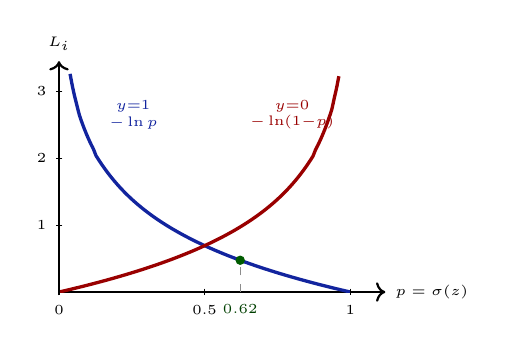
\begin{tikzpicture}[xscale=3.7,yscale=0.85]
        \draw[ax] (0,0)--(1.12,0) node[right,tlab]{$p=\sigma(z)$};
        \draw[ax] (0,-0.05)--(0,3.45) node[above,tlab]{$L_i$};
        \begin{scope}
          \clip (0,0) rectangle (1.04,3.3);
          % y=1 -> -ln(p): xato (p kichik) bo'lsa L katta
          \draw[curveA,domain=0.038:1] plot (\x,{-ln(\x)});
          % y=0 -> -ln(1-p)
          \draw[curveB,domain=0:0.962] plot (\x,{-ln(1-\x)});
        \end{scope}
        % I-slayd misoli: y=1, p=0.622 -> L=0.475
        \node[dotG] (ex) at (0.622,0.475) {};
        \draw[helperln] (0.622,0)--(0.622,0.475);
        \node[tlab,deepgreen!55!black,below=0pt] at (0.622,-0.04){$0.62$};
        % o'q belgilari
        \foreach \x/\l in {0/0,0.5/0.5,1/1}{%
          \draw (\x,0.05)--(\x,-0.05); \node[tlab,below] at (\x,-0.05){\l};}
        \foreach \y in {1,2,3}{%
          \draw (0.012,\y)--(-0.012,\y); \node[tlab,left] at (-0.01,\y){\y};}
        % egri nomlari
        \node[cnublue,tlab,align=center] at (0.255,2.65){$y{=}1$\\$-\ln p$};
        \node[deepred,tlab,align=center] at (0.80,2.65){$y{=}0$\\$-\ln(1{-}p)$};
      \end{tikzpicture}\\[1pt]
      {\scriptsize\textcolor{halfgray}{Ishonchli \alert{xato} $\Rightarrow$ $L$ portlaydi;
      to'g'ri $\Rightarrow$ $L\!\to\!0$.}}
    \end{column}
  \end{columns}
\end{frame}

% ----------------------------------------------------------------
% [H1b] CHIQARUV 2: gradient -> yangilash
% ----------------------------------------------------------------
\begin{frame}{LR ni keltirib chiqarish, 2-qism: gradient va uni yangilash qoidasi}
  \begin{columns}[T]
    \begin{column}{0.56\textwidth}
      \small
      \textbf{4-qadam.} $\sigma'(z)=\sigma(z)(1-\sigma(z))$ dan foydalanib:
      \[
        \frac{\partial L}{\partial w_j}
        \;=\;
        \frac{1}{N}\sum_{i=1}^{N}\bigl(\sigma(z_i)-y_i\bigr)\,x_{ij}
      \]
      \textcolor{halfgray}{\footnotesize
        intuitiv o'qilishi: ``bashorat xatosi'' $\times$ ``$j$-feature''}
      \pause

      \textbf{5-qadam.} SGD orqali yangilash ($\alpha$ = o'rganish tezligi):
      \[
        w_j \;\leftarrow\; w_j
        - \alpha\;\frac{\partial L}{\partial w_j}
      \]
      \vspace{2pt}
      \begin{tcolorbox}[okbox,title= SGD mantig'i]
        \footnotesize
        $\sigma(z_i)>y_i$ (ortiqcha baho)
        $\Rightarrow$ grad $>0$ $\Rightarrow$ $w_j\!\downarrow$.\\[2pt]
        $\sigma(z_i)<y_i$ (kam baho)
        $\Rightarrow$ grad $<0$ $\Rightarrow$ $w_j\!\uparrow$.
      \end{tcolorbox}
    \end{column}
    \begin{column}{0.42\textwidth}
      \centering
      % ---- Gradient descent: L(w) kosasi ----
      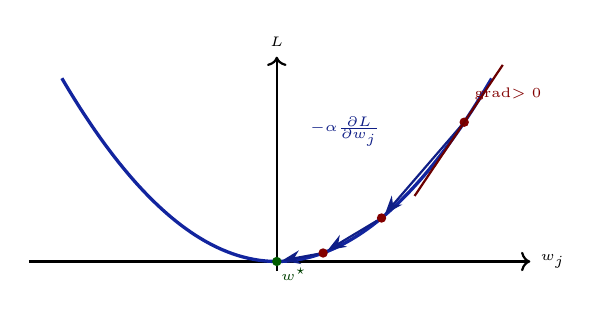
\begin{tikzpicture}[xscale=1.4,yscale=1.02]
        \draw[ax] (-2.25,0)--(2.3,0) node[right,tlab]{$w_j$};
        \draw[ax] (0,-0.12)--(0,2.55) node[above,tlab]{$L$};
        % parabola L(w)=0.6 w^2
        \draw[curveA,domain=-1.95:1.95] plot (\x,{0.6*\x*\x});
        % minimum
        \node[dotG] (m) at (0,0) {};
        \node[tlab,deepgreen!55!black,below right=-1pt and -2pt] at (0,0){$w^\star$};
        % tushish qadamlari (o'ngdan)
        \node[dotR] (p0) at (1.7,{0.6*1.7*1.7}) {};
        \node[dotR] (p1) at (0.95,{0.6*0.95*0.95}) {};
        \node[dotR] (p2) at (0.42,{0.6*0.42*0.42}) {};
        \draw[-Stealth,thick,cnublue!85!black] (p0)--(p1);
        \draw[-Stealth,thick,cnublue!85!black] (p1)--(p2);
        \draw[-Stealth,thick,cnublue!85!black] (p2)--(m);
        % boshlang'ich nuqtadagi nishab (gradient>0)
        \draw[deepred!70!black,thick] (1.25,{0.6*1.7*1.7-2.04*0.45})--(2.05,{0.6*1.7*1.7+2.04*0.35});
        \node[tlab,deepred!85!black,align=center,above right=-2pt and -3pt] at (1.78,1.95)
          {grad$>0$};
        \node[tlab,cnublue!85!black,align=center] at (0.62,1.62){$-\alpha\frac{\partial L}{\partial w_j}$};
      \end{tikzpicture}\\[1pt]
      {\scriptsize\textcolor{halfgray}{Har qadam $w_j$ ni $L$ minimumi sari suradi.}}
    \end{column}
  \end{columns}
\end{frame}

% ----------------------------------------------------------------
% [I1] QO'LDA MISOL: LR forward pass
% ----------------------------------------------------------------
\begin{frame}{LR ni qo'lda hisoblash}
  \small
  $\mathbf{x}=[\mathrm{TF\text{-}IDF(yaxshi)}{=}1.0,\;
  \mathrm{TF\text{-}IDF(yomon)}{=}0.0]$;\quad
  $\mathbf{w}=[0.8,\;{-}1.2]$,\; $b=-0.3$
  \vspace{5pt}
  \begin{columns}[T]
    \begin{column}{0.50\textwidth}
      \begin{tcolorbox}[defbox,title=Forward pass]
        \small
        $z = 0.8(1.0)+(-1.2)(0.0)+(-0.3) = 0.5$\\[5pt]
        $\sigma(0.5)=\dfrac{1}{1+e^{-0.5}}
        \approx\dfrac{1}{1.607}\approx 0.622$\\[5pt]
        $0.622>0.5$
        $\Rightarrow$ \textcolor{deepgreen}{\textbf{ijobiy}} \checkmark
      \end{tcolorbox}
    \end{column}
    \begin{column}{0.47\textwidth}
      \begin{tcolorbox}[defbox,title=Bitta namuna zarari ($y{=}1$)]
        \small
        $L_i = -\ln(0.622)\approx 0.475$\\[5pt]
        \textcolor{halfgray}{\footnotesize
          Noto'g'ri bashorat: $L_i$ oshadi.\\
          To'g'ri va ishonchli: $L_i$ kamayadi.}
      \end{tcolorbox}
    \end{column}
  \end{columns}
  \vspace{5pt}
  \textcolor{halfgray}{\footnotesize
    Eslatma: $e^{-0.5}\approx 0.607$;\quad
    kodda \texttt{from scipy.special import expit; expit(0.5)}.}
\end{frame}

% ----------------------------------------------------------------
% [J1] SIZNING VAZIFANGIZ: LR
% ----------------------------------------------------------------
\begin{frame}{Sizning vazifangiz: LR bashoratini hisoblang}
  \begin{tcolorbox}[warnbox,title=Vazifa (3 daqiqa)]
    \small
    Xuddi shu parametrlar:
    $\mathbf{w}=[0.8,\;{-}1.2]$,\; $b=-0.3$.\\[4pt]
    Yangi so'rov: $\mathbf{x}=[0,\;1]$
    \quad (faqat ``yomon'' so'zi uchraydi).\\[4pt]
    a)\; $z = ?$\qquad
    b)\; $\sigma(z)\approx ?$\quad ($e^{1.5}\approx 4.48$)\qquad
    c)\; Bashorat?
  \end{tcolorbox}
  \pause
  \begin{tcolorbox}[okbox,title=Javob]
    \small
    a)\; $z = 0.8(0)+(-1.2)(1)+(-0.3) = -1.5$\\[4pt]
    b)\; $\sigma(-1.5)=\dfrac{1}{1+e^{1.5}}
         \approx\dfrac{1}{5.48}\approx 0.182$\\[4pt]
    c)\; $0.182<0.5$
         $\Rightarrow$ \textcolor{deepred}{\textbf{salbiy}} \checkmark\quad
         \textcolor{halfgray}{\footnotesize
           (``yomon'' so'zi salbiy og'irlikka ega: $w_2=-1.2$)}
  \end{tcolorbox}
\end{frame}

% ----------------------------------------------------------------
% [K1] KOD <-> FORMULA: LogisticRegression  [fragile: lstlisting]
% ----------------------------------------------------------------
\begin{frame}[fragile]{Logistik regressiya kodi}
  \begin{columns}[T]
    \begin{column}{0.58\textwidth}
\begin{lstlisting}
from sklearn.pipeline import Pipeline
from sklearn.feature_extraction.text import TfidfVectorizer
from sklearn.linear_model import LogisticRegression

texts  = ["yaxshi mahsulot",
          "ajoyib sifat",
          "yomon yetkazish"]
labels = [1, 1, 0]

pipe = Pipeline([
    ('tfidf', TfidfVectorizer()),
    ('lr',   LogisticRegression(
                C=1.0,        # teskari C
                max_iter=200)),
])
pipe.fit(texts, labels)
p = pipe.predict_proba(["yaxshi mahsulot"])[0][1]
print(f"P(ijobiy) = {p:.3f}")
\end{lstlisting}
    \end{column}
    \begin{column}{0.39\textwidth}
      \small
      \begin{tabular}{@{}ll@{}}
        \toprule
        Kod & Formula \\
        \midrule
        \texttt{TfidfVectorizer} & $\mathbf{x}$ \\
        \texttt{C=1.0}           & teskari C\\
        \texttt{max\_iter}       & iteratsiyalar soni\\
        \texttt{predict\_proba}  & $\sigma(\mathbf{w}\cdot\mathbf{x}+b)$ \\
        \texttt{predict}         & $>0.5$? \\
        \bottomrule
      \end{tabular}
      \vspace{6pt}\\
      \small\textbf{Muhim:}\\
      \texttt{C} kichik bo'lsa $\Rightarrow$\\
      ko'proq regularizatsiya\\
      (vaznlar kichrayadi)
    \end{column}
  \end{columns}
\end{frame}

% ----------------------------------------------------------------
% [L1] TUZOG': tengsiz ma'lumot
% ----------------------------------------------------------------
\begin{frame}{LR da sinflar nomutanosibligi (class imbalance)}
  \begin{tcolorbox}[warnbox,title=Muammo]
    \small
    O'quv ma'lumotlari: 900 salbiy, 100 ijobiy sharh.\\
    Oddiy LR modeli deyarli barcha namunalarni ``salbiy'' deb bashorat qilishni o'rganishi mumkin.\\
    Natija: \texttt{accuracy=90\%}, lekin \texttt{F1=0\%}
    --- butunlay foydasiz model!
  \end{tcolorbox}
  \vspace{6pt}
  \begin{tcolorbox}[okbox,title={Yechim: \texttt{class\_weight='balanced'}}]
    \small
    \texttt{LogisticRegression(class\_weight='balanced')}\\[4pt]
    Avtomatik og'irlik:\quad
    $w_c = \dfrac{N}{K\,n_c}$\\[2pt]
    \footnotesize $N$ --- jami namunalar, $K$ --- sinflar soni,
    $n_c$ --- $c$ sinfidagi namunalar soni.\\[2pt]
    \textcolor{halfgray}{\footnotesize
      Kam sinfga ko'proq og'irlik beriladi; macro $F_1$ validatsiyada tekshiriladi.\\
      Alternativ usul: oversampling yoki threshold tuning.}
  \end{tcolorbox}
  \vspace{4pt}
  \small\textcolor{halfgray}{F1 metrikasini quyida muhokama qilamiz.}
\end{frame}

% ================================================================
\section[Naive Bayes]{Naive Bayes + Laplace silliqlash}
% ================================================================

% ----------------------------------------------------------------
% [F2] INTUITSIYA: sanash bilan tasniflash
% ----------------------------------------------------------------
\begin{frame}{Naive Bayes: sanashga asoslangan ehtimollik modeli}
  \begin{columns}[T]
    \begin{column}{0.50\textwidth}
      \small
      \textbf{Savol:} ``yaxshi film'' ijobiy sharh deganimi?\\[5pt]
      \textbf{NB javobi:} O'quv ma'lumotlarida ``yaxshi'' so'zi
      ijobiy matnlarda \textit{necha marta} uchragan?
      Salbiy matnlarda-chi?\\[5pt]
      $\to$ sanab chiqamiz $\to$ ehtimollikni hisoblaymiz $\to$ taqqoslaymiz\\[5pt]
      \begin{tcolorbox}[defbox,title=NB mantig'i]
        \small
        LR: $P(y|\mathbf{x})$ --- qaror chegarasini to'g'ridan-to'g'ri o'rganadi\\
        (diskriminativ model)\\[3pt]
        NB: $P(\mathbf{x}|y)P(y)$ --- har sinfni modellaydi\\
        (generativ model)
      \end{tcolorbox}
    \end{column}
    \begin{column}{0.46\textwidth}
      \small
      \textbf{Afzalliklari:}\\[4pt]
      \begin{tabular}{@{}lll@{}}
        \toprule
        & LR & NB \\
        \midrule
        O'qitish & iterativ & sanash orqali tez \\
        Kichik data & regularizatsiya kerak & barqaror \\
        Talqin & $w_j$ & $P(w|y)$ \\
        \bottomrule
      \end{tabular}
      \vspace{6pt}\\
      \small\textcolor{halfgray}{
        O'zbek tili uchun:\\
        kichik korpusda NB barqaror natija beradi,\\
        korpus hajmi o'sganda LR ham yaxshilanadi.}
    \end{column}
  \end{columns}
\end{frame}

% ----------------------------------------------------------------
% [G2] RASMIY TA'RIF: Bayes teoremasi + CI + bunda
% ----------------------------------------------------------------
\begin{frame}{Naive Bayes: Bayes teoremasi va uning sodda farazi}
  \begin{columns}[T]
    \begin{column}{0.49\textwidth}
      \begin{tcolorbox}[defbox,title=Bayes teoremasi]
        \[
          P(y\mid\mathbf{x})
          \;\propto\;
          P(\mathbf{x}\mid y)\,P(y)
        \]
      \end{tcolorbox}
      \vspace{1pt}
      \begin{tcolorbox}[defbox,title=``Naive'' --- shartli mustaqillik]
        \[
          P(\mathbf{x}\mid y)
          \;\propto\;
          \prod_{j=1}^{|V|} P(w_j\mid y)^{x_j}
        \]
        \scriptsize\textcolor{halfgray}{
          $x_j$ --- $w_j$ ning sanog'i; so'zlar sinf berilganda shartli mustaqil deb
          faraz qilinadi (amalda ko'pincha buziladi).}
      \end{tcolorbox}
    \end{column}
    \begin{column}{0.50\textwidth}
      \centering
      % ---- Prior x Likelihood -> Posterior ----
      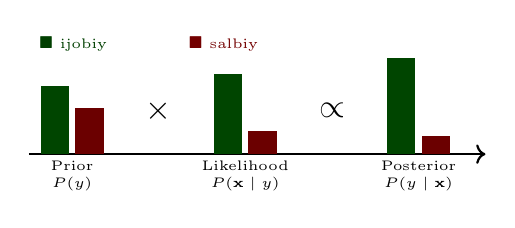
\begin{tikzpicture}[font=\tiny]
        \def\H{1.45}
        \draw[ax] (-0.55,0)--(5.25,0);
        % --- guruh chizish: cx, h_pos, h_neg ---
        \foreach \cx/\hp/\hn in {0/0.6/0.4, 2.2/0.7/0.2, 4.4/0.84/0.16}{
          \fill[deepgreen!60!black] (\cx-0.40,0) rectangle (\cx-0.04,{\hp*\H});
          \fill[deepred!70!black]   (\cx+0.04,0) rectangle (\cx+0.40,{\hn*\H});
        }
        % operatorlar
        \node[font=\large] at (1.1,0.55){$\times$};
        \node[font=\large] at (3.3,0.55){$\propto$};
        % guruh nomlari
        \node[align=center] at (0,-0.28){Prior\\$P(y)$};
        \node[align=center] at (2.2,-0.28){Likelihood\\$P(\mathbf{x}\mid y)$};
        \node[align=center] at (4.4,-0.28){Posterior\\$P(y\mid\mathbf{x})$};
        % legend
        \node[deepgreen!55!black,right] at (-0.55,1.4){$\blacksquare$ ijobiy};
        \node[deepred!75!black,right]  at (1.35,1.4){$\blacksquare$ salbiy};
      \end{tikzpicture}\\[6pt]
      {\scriptsize\textcolor{halfgray}{Dalil (so'zlar) priorni qayta tortadi
      $\Rightarrow$ posterior keskinlashadi.}}
    \end{column}
  \end{columns}
  \vspace{3pt}
  \bunda{%
    \footnotesize $P(y)$ = prior;\;
    $P(\mathbf{x}|y)$ = likelihood;\;
    $P(y|\mathbf{x})$ = posterior;\;
    $|V|$ = lug'at hajmi%
  }
\end{frame}

% ----------------------------------------------------------------
% [H2a] CHIQARUV 1: ko'paytma -> log-space
% ----------------------------------------------------------------
\begin{frame}{NB ni keltirib chiqarish, 1-qism:}
  \begin{columns}[T]
    \begin{column}{0.58\textwidth}
      \small
      \textbf{1-qadam.} NB tasniflash qoidasi:
      \[
        \hat{y}
        =\operatorname*{arg\,max}_{y}
        \Bigl[P(y)\prod_{j=1}^{|V|}P(w_j\mid y)^{x_j}\Bigr]
      \]
      \pause
      \textbf{2-qadam.} Logarifmga o'tish
      (monoton $\Rightarrow$ $\operatorname{arg\,max}$ o'zgarmaydi):
      \[
        \hat{y}
        =\operatorname*{arg\,max}_{y}
        \Bigl[\log P(y) + \sum_{j=1}^{|V|}x_j\log P(w_j\mid y)\Bigr]
      \]
      \pause
      \begin{tcolorbox}[warnbox,title=Nima uchun log?]
        \footnotesize
        100 ta so'z, har biri $P\!\approx\!0.01$:\\
        $0.01^{100}=10^{-200}$ --- Python da \texttt{0.0}
        (\textit{underflow} xavfi!)\\
        Log bilan: $100\times\log(0.01)=-460$ --- xavfsiz.
      \end{tcolorbox}
    \end{column}
    \begin{column}{0.41\textwidth}
      \centering
      % ---- log kichik ehtimollikni xavfsiz oraliqqa "cho'zadi" ----
      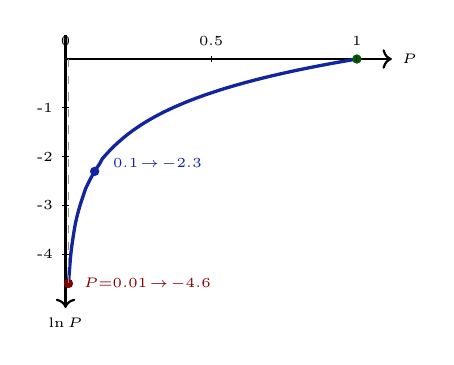
\begin{tikzpicture}[xscale=3.7,yscale=0.62]
        \draw[ax] (0,0)--(1.12,0) node[right,tlab]{$P$};
        \draw[ax] (0,0.5)--(0,-5.1) node[below,tlab]{$\ln P$};
        \draw[curveA,domain=0.0095:1] plot (\x,{ln(\x)});
        % belgilangan nuqtalar
        \node[dotR] (a) at (0.01,{ln(0.01)}) {};
        \draw[helperln] (0.01,0)--(0.01,{ln(0.01)});
        \node[tlab,deepred!85!black,right=1pt] at (0.02,{ln(0.01)}){$P{=}0.01\!\to\!-4.6$};
        \node[dotB] at (0.1,{ln(0.1)}) {};
        \node[tlab,cnublue,right=1pt] at (0.12,{ln(0.1)+0.15}){$0.1\!\to\!-2.3$};
        \node[dotG] at (1,0) {};
        % belgilar
        \foreach \x/\l in {0/0,0.5/0.5,1/1}{%
          \draw (\x,0.07)--(\x,-0.07); \node[tlab,above] at (\x,0.07){\l};}
        \foreach \y in {-1,-2,-3,-4}{%
          \draw (0.012,\y)--(-0.012,\y); \node[tlab,left] at (-0.01,\y){\y};}
      \end{tikzpicture}\\[1pt]
      {\scriptsize\textcolor{halfgray}{Kichik $P\!\in\!(0,1)$ $\to$ chekli manfiy son;
      ko'paytma $\Rightarrow$ \alert{yig'indi}.}}
    \end{column}
  \end{columns}
\end{frame}

% ----------------------------------------------------------------
% [H2b] CHIQARUV 2: nol chastota -> Laplace
% ----------------------------------------------------------------
\begin{frame}{NB ni keltirib chiqarish, 2-qism: Laplace (Add-$\alpha$) silliqlash}
  \begin{columns}[T]
    \begin{column}{0.54\textwidth}
      \begin{tcolorbox}[warnbox,title=0 marta uchrash muammosi]
        \footnotesize
        ``ajoyib'' so'zi \textit{salbiy} sinfda 0 marta uchrasa:\\
        $P(\text{ajoyib}|\text{neg})=0$
        $\Rightarrow$ butun ko'paytma $=0$
        $\Rightarrow$ model ishlamaydi!
      \end{tcolorbox}
      \vspace{3pt}
      \begin{tcolorbox}[defbox,title=Laplace silliqlash formulasi]
        \[
          P(w\mid y)
          \;=\;
          \frac{\mathrm{count}(w,y)+\alpha}{N_y+\alpha\,|V|}
        \]
      \end{tcolorbox}
      \vspace{2pt}
      \footnotesize
      \textcolor{halfgray}{$\alpha{=}0$ silliqlashsiz;\;
      $\alpha{=}1$ Laplace;\;
      $\alpha{\gg}1$ barcha so'zlar teng.}
    \end{column}
    \begin{column}{0.44\textwidth}
      \centering
      % ---- alpha ta'siri: P(ajoyib|neg) = alpha/(2+4 alpha) ----
      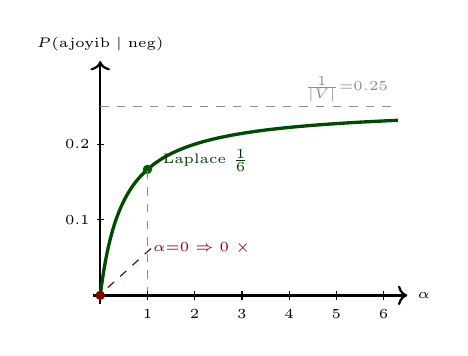
\begin{tikzpicture}[xscale=0.6,yscale=9.6]
        \draw[ax] (-0.15,0)--(6.5,0) node[right,tlab]{$\alpha$};
        \draw[ax] (0,-0.012)--(0,0.31) node[above,tlab]{$P(\text{ajoyib}\mid\text{neg})$};
        % asimptota 1/|V|=0.25
        \draw[helperln] (0,0.25)--(6.3,0.25);
        \node[tlab,halfgray,above left=-2pt and 0pt] at (6.3,0.25){$\tfrac{1}{|V|}{=}0.25$};
        \draw[curveC,domain=0:6.3] plot (\x,{\x/(2+4*\x)});
        % alpha=0 -> 0
        \node[dotR] (z0) at (0,0){};
        \node[tlab,deepred!85!black,fill=white,inner sep=0.6pt] (z0l) at (2.15,0.062){$\alpha{=}0\Rightarrow 0$ \alert{$\times$}};
        \draw[helperln,deepred!55!black] (z0l.west)--(0.05,0.004);
        % alpha=1 -> 1/6
        \node[dotG] at (1,{1/6}){};
        \draw[helperln] (1,0)--(1,{1/6});
        \node[tlab,deepgreen!50!black,right=2pt] at (1,{1/6+0.012}){Laplace $\tfrac{1}{6}$};
        \foreach \x in {1,2,3,4,5,6}{\draw (\x,0.006)--(\x,-0.006); \node[tlab,below] at (\x,-0.006){\x};}
        \foreach \y/\l in {0.1/0.1,0.2/0.2}{%
          \draw (0.07,\y)--(-0.07,\y); \node[tlab,left] at (-0.02,\y){\l};}
      \end{tikzpicture}\\[1pt]
      {\scriptsize\textcolor{halfgray}{$\alpha$ nolni ko'taradi; juda katta $\alpha$ teng taqsimotga itaradi.}}
    \end{column}
  \end{columns}
  \vspace{2pt}
  \bunda{%
    \footnotesize $\mathrm{count}(w,y)$ = $w$ uchrashlar soni;\;
    $N_y$ = $y$ sinfdagi tokenlar;\;
    $|V|$ = lug'at hajmi;\;
    $\alpha{=}1$ = Laplace%
  }
\end{frame}

% ----------------------------------------------------------------
% [I2] LOCKED QO'LDA HISOB --- P2 birinchi assert manbayi
%
% P2 (kun 3) assert:
%   score_pos = (2/3)(1/4)(3/8) = 6/96 = 1/16 = 0.0625
%   score_neg = (1/3)(1/6)(1/3) = 2/108 = 1/54 ≈ 0.0185
%   ratio = (1/16)/(1/54) = 54/16 = 27/8 = 3.375
%   assert abs(ratio - 3.375) < 0.01   # Ma'ruza L2 [I2]-slayd
% ----------------------------------------------------------------
\begin{frame}{Naive Bayes asosida tasniflashni qo'lda hisoblaymiz}
  \small
  \textbf{O'quv to'plami:}\;
  pos=[\,``yaxshi film'',``ajoyib film''\,],\;
  neg=[\,``yomon film''\,]\\[2pt]
  $|V|{=}4$\;$\{$yaxshi, ajoyib, yomon, film$\}$;\quad
  $P(\text{pos}){=}2/3$,\; $P(\text{neg}){=}1/3$
  \vspace{5pt}
  \begin{columns}[T]
    \begin{column}{0.52\textwidth}
      \textbf{Laplace ($\alpha{=}1$):}\\[3pt]
      \footnotesize
      \begin{tabular}{@{}lll@{}}
        \toprule
        $P(w|y)$ & pos\;($N_y{=}4$) & neg\;($N_y{=}2$) \\
        \midrule
        film   & $(2{+}1)/(4{+}4)=3/8$ & $(1{+}1)/(2{+}4)=1/3$ \\
        yaxshi & $(1{+}1)/(4{+}4)=1/4$ &
                 \alert{$(0{+}1)/(2{+}4)=1/6$} \\
        \bottomrule
      \end{tabular}\\[3pt]
      \textcolor{halfgray}{\tiny
        \alert{$1/6$}: nol chastota $\to$ Laplace natijasi}
    \end{column}
    \begin{column}{0.45\textwidth}
      \textbf{Test: ``yaxshi film''}\\[3pt]
      \small
      \begin{align*}
        \text{s}_{\text{pos}}
          &=\tfrac{2}{3}\cdot\tfrac{1}{4}\cdot\tfrac{3}{8}
          =\tfrac{6}{96}=\tfrac{1}{16}\approx 0.0625\\[4pt]
        \text{s}_{\text{neg}}
          &=\tfrac{1}{3}\cdot\tfrac{1}{6}\cdot\tfrac{1}{3}
          =\tfrac{2}{108}=\tfrac{1}{54}\approx 0.0185
      \end{align*}
      \[
        \text{nisbat}
        =\frac{1/16}{1/54}
        =\frac{54}{16}
        =\frac{27}{8}
        =\mathbf{3.375}
        \;\to\;\textcolor{deepgreen}{\textbf{ijobiy}}
      \]
      \footnotesize\textcolor{halfgray}{%
        2-amaliyotda assert:\;\texttt{abs(ratio-3.375)<0.01} ga duch kelasiz}
    \end{column}
  \end{columns}
\end{frame}

% ----------------------------------------------------------------
% [J2] SIZNING VAZIFANGIZ: NB
% ----------------------------------------------------------------
\begin{frame}{Sizning vazifangiz: Naive Bayes asosida tasniflashni qo'lda hisoblang}
  \begin{tcolorbox}[warnbox,title=Vazifa (4 daqiqa)]
    \small
    Xuddi shu korpus (hozirgina ko'rgan misolimiz). 
    \textbf{``yomon''} so'zi (bitta so'z, $\alpha{=}1$) uchun Naive Bayes orqali quyidagilarni hisoblang:\\[4pt]
    a)\; $P(\text{yomon}|\text{pos}) = ?$\qquad
    b)\; $P(\text{yomon}|\text{neg}) = ?$\\[4pt]
    c)\; $\text{score}_\text{pos}$ va $\text{score}_\text{neg}$.\quad
    d)\; nisbat $<1$ yoki $>1$?\; Qaysi sinf?
  \end{tcolorbox}
  \pause
  \begin{tcolorbox}[okbox,title=Javob]
    \small
    a)\; $P(\text{yomon}|\text{pos})=(0{+}1)/(4{+}4)=1/8$
         \;\textcolor{halfgray}{\footnotesize (nol chastota!)}\\[4pt]
    b)\; $P(\text{yomon}|\text{neg})=(1{+}1)/(2{+}4)=2/6=1/3$\\[4pt]
    c)\; $\text{s}_\text{pos}=(2/3)(1/8)=1/12\approx 0.083$;\;
         $\text{s}_\text{neg}=(1/3)(1/3)=1/9\approx 0.111$\\[4pt]
    d)\; nisbat $=(1/12)/(1/9)=9/12=3/4=0.75<1$
         $\Rightarrow$ \textcolor{deepred}{\textbf{salbiy}} \checkmark
  \end{tcolorbox}
\end{frame}

% ----------------------------------------------------------------
% [K2] KOD <-> FORMULA: MultinomialNB  [fragile: lstlisting]
% ----------------------------------------------------------------
\begin{frame}[fragile]{Naive Bayesni kodda ishlatish}
  \begin{columns}[T]
    \begin{column}{0.57\textwidth}
\begin{lstlisting}
from sklearn.feature_extraction.text import (
    CountVectorizer)
from sklearn.naive_bayes import MultinomialNB

korpus = [
    "yaxshi film",  # ijobiy (1)
    "ajoyib film",  # ijobiy (1)
    "yomon film",   # salbiy (0)
]
labels = [1, 1, 0]

vec = CountVectorizer()
X   = vec.fit_transform(korpus)

nb  = MultinomialNB(alpha=1.0)  # Laplace
nb.fit(X, labels)

test  = vec.transform(["yaxshi film"])
proba = nb.predict_proba(test)
# proba[0] = [P(salbiy), P(ijobiy)]
print(f"P(ijobiy) = {proba[0][1]:.4f}")
\end{lstlisting}
    \end{column}
    \begin{column}{0.40\textwidth}
      \small
      \begin{tabular}{@{}ll@{}}
        \toprule
        Kod & Formula \\
        \midrule
        \texttt{alpha=1.0} & $\alpha$ (Laplace) \\
        \texttt{fit\_transform} & $\mathrm{count}(w,y)$, $N_y$ \\
        \texttt{predict\_proba} & log$\sum$ $\to$ exp\\
        \texttt{predict}        & $\operatorname{arg\,max}$ \\
        \bottomrule
      \end{tabular}
      \vspace{6pt}\\
      \small\textbf{Tekshirib ko'ring:}\\
      \texttt{nb.feature\_log\_prob\_}\\
      $\to\log P(w|y)$ matritsasi natijasini beradi\\[4pt]
      \textcolor{halfgray}{\footnotesize
        Nisbatni olish:\\
        \texttt{np.exp(}\\
        \texttt{~~log\_sp - log\_sn)}}
    \end{column}
  \end{columns}
\end{frame}

% ----------------------------------------------------------------
% [L2] TUZOG': korrelyatsiyali belgilar
% ----------------------------------------------------------------
\begin{frame}{Naive Bayesda korrelyatsiyalangan xususiyatlar muammosi}
  \begin{tcolorbox}[warnbox,title=Shartli mustaqillik farazi buzilish muammosi:]
    \small
    ``juda yaxshi'' $\to$ ``juda'' va ``yaxshi'' birga uchraydi.\\
    Naive Bayes (NB) ikkisini \textbf{mustaqil} hisoblaydi
    $\to$ ijobiy sinf uchun hisoblash jarayonida yaxshi so'zi \textbf{ikki marta} sanaladi, model ehtimollikni sun'iy ravishda oshirib yuboradi va ortiqcha ishonchli bashoratga olib keladi.\\[4pt]
    ``Sifati yaxshi, sifatli mahsulot'' jumlasida bir ildizga yaqin so'zlar model signalini takrorlashi mumkin.
  \end{tcolorbox}
  \vspace{5pt}
  \begin{tcolorbox}[okbox,title=Yechimlar]
    \small
    \begin{enumerate}
      \item \textbf{Binary xususiyatlar:} \\
            \texttt{CountVectorizer(binary=True)}
      \item \textbf{Logistik regressiya bilan bashorat qilish:} u korrelyatsiyalangan belgilarga odatda bardoshliroq.
      \item \textbf{N-gram}lar orqali ``juda yaxshi'' ni bitta tokenga aylantirish.
    \end{enumerate}
  \end{tcolorbox}
\end{frame}


% ----------------------------------------------------------------
% [L2b] TUZOG': data leakage
% ----------------------------------------------------------------
\begin{frame}{train-test to'plamlarida ma'lumotlar sizib o'tishi (leakage)}
  \begin{tcolorbox}[warnbox,title=Noto'g'ri tartib]
    \footnotesize
    1) Avval butun korpusda \texttt{TfidfVectorizer.fit()} qilish;\\
    2) keyin train/testga bo'lish.\\[2pt]
    Natijada, test ma'lumotidagi so'zlar umumiy ma'lumot ichida IDFga kirib ketadi, model test ma'lumotlari taqsimotini oldindan ko'radi va model aniqligi sun'iy oshadi.
  \end{tcolorbox}
  \begin{tcolorbox}[okbox,title=To'g'ri tartib]
    \footnotesize
    \texttt{train\_test\_split(..., stratify=y)} $\to$
    \texttt{Pipeline([('tfidf', TfidfVectorizer()), ('clf', model)])} $\to$
    \texttt{pipe.fit(X\_train, y\_train)} $\to$
    \texttt{pipe.predict(X\_test)}.\\[2pt]
    Amaliy qoida: preprocessing va vektorizatsiya parametrlari \textbf{faqat train} to'plamdan o'rganiladi.
  \end{tcolorbox}
  \textcolor{halfgray}{\footnotesize 2-amaliyotda Logistik regressiya (LR) va Naive Bayes (NB) aynan \texttt{Pipeline} ichida solishtiriladi.}
\end{frame}

% ================================================================
\section[Metrikalar]{Modelni baholash}
% ================================================================

% ----------------------------------------------------------------
% [F3] INTUITSIYA: accuracy aldaydi
% ----------------------------------------------------------------
\begin{frame}{Model natijasini baholash uchun nima uchun accuracy yetarli emas?}
  \begin{columns}[T]
    \begin{column}{0.53\textwidth}
      \small
      \textbf{Muammo:} 1000 sharh, 900 salbiy, 100 ijobiy.\\[6pt]
      \textbf{Model A} sharhlarni o'rganish jarayonida aksariyat holda salbiy sharhni ko'rdi va u yangi sharhni testlashda \textit{``salbiy'' deb tasniflash ehtimoli yuqori.}\\[5pt]
      \begin{tcolorbox}[warnbox]
        \small
        Accuracy $= 900/1000 = \mathbf{90\%}$\\[2pt]
        Lekin: 100 ijobiy sharhning
        \textbf{birortasini} to'g'ri topmadi!
      \end{tcolorbox}
    \end{column}
    \begin{column}{0.43\textwidth}
      \vspace{8pt}
      \begin{tcolorbox}[defbox,title=Muammo]
        \small
        Kompaniyaning ``90\% aniqlik''da ishlaydigan modeli
        aslida ijobiy sharh yozgan mijozlarga g'alati ko'rinadi.\\[4pt]
        Raqamlar aldaydi ---
        bizga \textbf{muvozanatli}
        metrika kerak.
      \end{tcolorbox}
    \end{column}
  \end{columns}
\end{frame}

% ----------------------------------------------------------------
% [G3] CONFUSION MATRIX + 4 METRIKA + BUNDA
% ----------------------------------------------------------------
\begin{frame}{Confusion matrix va to'rt metrika}
  \begin{columns}[T]
    \begin{column}{0.44\textwidth}
      \centering
      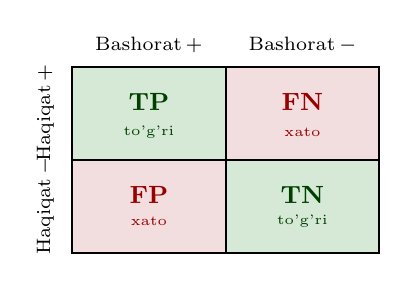
\begin{tikzpicture}[font=\small]
        \def\cw{1.95}\def\ch{1.18}
        % --- diagonal = to'g'ri (yashil), diagonaldan tashqari = xato (qizil) ---
        \fill[deepgreen!16] (0,0)     rectangle (\cw,\ch);     % TP
        \fill[deepred!13]   (\cw,0)   rectangle (2*\cw,\ch);   % FN
        \fill[deepred!13]   (0,-\ch)  rectangle (\cw,0);       % FP
        \fill[deepgreen!16] (\cw,-\ch)rectangle (2*\cw,0);     % TN
        \draw[thick] (0,-\ch) rectangle (2*\cw,\ch);
        \draw[thick] (\cw,-\ch) -- (\cw,\ch);
        \draw[thick] (0,0) -- (2*\cw,0);
        % cell labels (har katakda: katta belgi tepada, izoh pastda)
        \node[deepgreen!55!black] at (0.5*\cw, 0.62*\ch) {\textbf{TP}};
        \node[tlab,deepgreen!55!black] at (0.5*\cw, 0.30*\ch){to'g'ri};
        \node[deepred]            at (1.5*\cw, 0.62*\ch) {\textbf{FN}};
        \node[tlab,deepred]       at (1.5*\cw, 0.30*\ch){xato};
        \node[deepred]            at (0.5*\cw,-0.38*\ch) {\textbf{FP}};
        \node[tlab,deepred]       at (0.5*\cw,-0.66*\ch){xato};
        \node[deepgreen!55!black] at (1.5*\cw,-0.38*\ch) {\textbf{TN}};
        \node[tlab,deepgreen!55!black] at (1.5*\cw,-0.66*\ch){to'g'ri};
        % column headers (bashorat)
        \node[font=\scriptsize] at (0.5*\cw,\ch+0.28) {Bashorat\,+};
        \node[font=\scriptsize] at (1.5*\cw,\ch+0.28) {Bashorat\,$-$};
        % row headers (haqiqat)
        \node[font=\scriptsize,rotate=90] at (-0.34, 0.5*\ch) {Haqiqat\,+};
        \node[font=\scriptsize,rotate=90] at (-0.34,-0.5*\ch) {Haqiqat\,$-$};
      \end{tikzpicture}

      \vspace{5pt}
      {\footnotesize
       \textcolor{deepgreen!55!black}{$\blacksquare$} diagonal = to'g'ri bashorat \,(TP, TN)\\
       \textcolor{deepred}{$\blacksquare$} tashqarisi = xato \,(FP --- noto'g'ri ijobiy; FN --- o'tkazib yuborilgan)}
    \end{column}
    \begin{column}{0.53\textwidth}
      \begin{tcolorbox}[defbox,title=To'rt metrika]
        \small
        \[
          Accuracy= \frac{TP+TN}{TP+TN+FP+FN}
        \]
        \[
          Precision = \frac{TP}{TP+FP}
          \qquad
          Recall = \frac{TP}{TP+FN}
        \]
        \[
          F_1 score= \frac{2PR}{P+R}
              = \frac{2\,TP}{2\,TP+FP+FN}
        \]
      \end{tcolorbox}
    \end{column}
  \end{columns}
\end{frame}

% ----------------------------------------------------------------
% [H3a] CHIQARUV: precision va recall ma'nosi
% ----------------------------------------------------------------
\begin{frame}{Precision va recall: qachon qaysi biri muhim?}
  \begin{columns}[T]
    \begin{column}{0.49\textwidth}
      \begin{tcolorbox}[defbox,title={Precision $P=TP/(TP{+}FP)$}]
        \small
        Precision: ``ijobiy deganlarimizning qanchasi haqiqatan ijobiy?''\\[4pt]
        \textbf{Spam filtri modeli qursangiz va  FP yuqori bo'lsa, bu yomon (muhim xat spam
        deb belgilanadi).}
      \end{tcolorbox}
    \end{column}
    \begin{column}{0.49\textwidth}
      \begin{tcolorbox}[defbox,title={Recall $R=TP/(TP{+}FN)$}]
        \small
        Recall: ``Haqiqiy ijobiylarning qanchasini topdim?''\\[4pt]
        \textbf{Tibbiy diagnoz qiluvchi model qursangiz va FN yuqori bo'lsa, bu yomon (kasallikni
        o'tkazib yuborish).}
      \end{tcolorbox}
    \end{column}
  \end{columns}
  \vspace{5pt}
  \begin{columns}[T]
    \begin{column}{0.53\textwidth}
      \begin{tcolorbox}[warnbox,title=Savdoning ikki tomoni]
        \footnotesize
        Qaror chegarasi oshsa odatda $P\!\uparrow$, $R\!\downarrow$; chegara pasaysa aksincha.\\[2pt]
        $F_1$ --- precision va recallning \textbf{garmonik o'rtachasi}; ikkalasini birga baholaydi.
      \end{tcolorbox}
    \end{column}
    \begin{column}{0.45\textwidth}
      \centering
      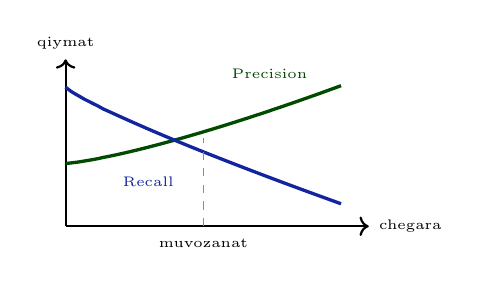
\begin{tikzpicture}[font=\tiny]
        \def\W{3.5}\def\H{1.9}
        \draw[ax] (0,0) -- (\W+0.35,0) node[right,font=\tiny]{chegara};
        \draw[ax] (0,0) -- (0,\H+0.22)  node[above,font=\tiny]{qiymat};
        % precision rises with threshold (yashil)
        \draw[curveC,domain=0:1,samples=60]
              plot (\x*\W,{(0.42+0.52*pow(\x,1.3))*\H});
        % recall falls with threshold (ko'k)
        \draw[curveA,domain=0:1,samples=60]
              plot (\x*\W,{(0.93-0.78*pow(\x,0.85))*\H});
        \node[deepgreen!60!black] at (\W*0.74,\H*1.02) {Precision};
        \node[cnublue]            at (\W*0.30,\H*0.30) {Recall};
        % kesishish (muvozanat)
        \draw[helperln] (\W*0.5,0) -- (\W*0.5,\H*0.59);
        \node[tlab] at (\W*0.5,-0.22) {muvozanat};
      \end{tikzpicture}
    \end{column}
  \end{columns}
\end{frame}

% ----------------------------------------------------------------
% [H3b] CHIQARUV: F1 garmonik; imbalance kontrast jadvali
% ----------------------------------------------------------------
\begin{frame}{$F_1$ score}
  \small
  \textbf{Nima uchun garmonik, arifmetik emas?}\\[3pt]
  \begin{columns}[T]
    \begin{column}{0.55\textwidth}
      $P{=}0.90$, $R{=}0.10$ bo'lsa (model juda oz ijobiyni topgan):\\[6pt]
      Arifmetik: $(0.90+0.10)/2=0.50$\\
      \quad--- o'rtacha (hammasi yaxshiday).\; \alert{Aldaydi!}\\[6pt]
      Garmonik:
      $F_1=\dfrac{2(0.90)(0.10)}{0.90+0.10}=\mathbf{0.18}$\\
      \quad--- past natija \checkmark
    \end{column}
    \begin{column}{0.44\textwidth}
      \centering
      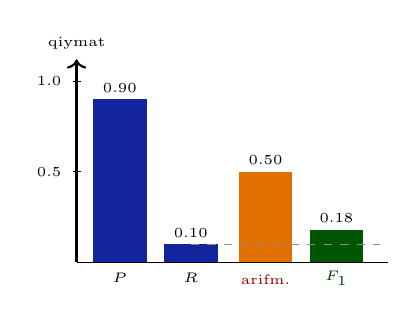
\begin{tikzpicture}[font=\tiny]
        \def\H{2.3}\def\bw{0.34}
        \draw[ax] (0,0) -- (0,\H+0.28) node[above]{qiymat};
        \draw[thin] (-0.05,\H)-- (0.05,\H);
          \node[tlab,left] at (-0.07,\H){1.0};
        \draw[thin] (-0.05,0.5*\H)-- (0.05,0.5*\H);
          \node[tlab,left] at (-0.07,0.5*\H){0.5};
        \draw[thin] (0,0) -- (3.95,0);
        % P = 0.90
        \fill[cnublue] (0.55-\bw,0) rectangle (0.55+\bw,0.90*\H);
        \node[tlab] at (0.55,0.90*\H+0.15){0.90}; \node[tlab] at (0.55,-0.2){$P$};
        % R = 0.10
        \fill[cnublue] (1.45-\bw,0) rectangle (1.45+\bw,0.10*\H);
        \node[tlab] at (1.45,0.10*\H+0.15){0.10}; \node[tlab] at (1.45,-0.2){$R$};
        % arifmetik = 0.50 (aldaydi)
        \fill[orange!88!black] (2.4-\bw,0) rectangle (2.4+\bw,0.50*\H);
        \node[tlab] at (2.4,0.50*\H+0.15){0.50};
        \node[tlab,deepred] at (2.4,-0.22){arifm.};
        % F1 garmonik = 0.18
        \fill[deepgreen!75!black] (3.3-\bw,0) rectangle (3.3+\bw,0.18*\H);
        \node[tlab] at (3.3,0.18*\H+0.15){0.18};
        \node[tlab,deepgreen!55!black] at (3.3,-0.20){$F_1$};
        % R darajasi: F1 kichik qiymatga yaqin turishini ko'rsatadi
        \draw[helperln] (1.45,0.10*\H) -- (3.85,0.10*\H);
      \end{tikzpicture}
    \end{column}
  \end{columns}
  \vspace{1pt}
  \begin{tcolorbox}[defbox,title=Ikki model taqqoslash (900 salbiy / 100 ijobiy)]
    \footnotesize
    \begin{tabular}{@{}lcccc@{}}
      \toprule
      Model & Accuracy & Precision & Recall & $F_1$ \\
      \midrule
      A (hammasi salbiy) &
        $90\%$ & --- & $0\%$ & \textcolor{deepred}{$0\%$} \\
      B (o'rgangan;\; TP=60, FP=80, FN=40) &
        $88\%$ & $43\%$ & $60\%$ &
        \textcolor{deepgreen}{$\approx\!50\%$} \\
      \bottomrule
    \end{tabular}
    \vspace{2pt}\\
    \textcolor{halfgray}{Model A accuracy yuqori,
    lekin $F_1{=}0$ --- butunlay foydasiz!}
  \end{tcolorbox}
\end{frame}

% ----------------------------------------------------------------
% [I3] QO'LDA HISOB: Model B confusion matrix -> metrikalar
% ----------------------------------------------------------------
\begin{frame}{Confusion matrixdan metrikalarni qo'lda hisoblab olish}
  \small
  \textbf{Model B:}\;
  TP=60,\; TN=820,\; FP=80,\; FN=40\quad (jami 1000)
  \vspace{5pt}
  \begin{columns}[T]
    \begin{column}{0.50\textwidth}
      \begin{tcolorbox}[defbox,title=Hisoblar (qo'lda)]
        \small
        $A=(60+820)/1000=0.88$\\[4pt]
        $P=60/(60+80)=60/140\approx 0.429$\\[4pt]
        $R=60/(60+40)=60/100=0.600$\\[4pt]
        $F_1=\dfrac{2(0.429)(0.600)}{0.429+0.600}$\\[4pt]
        $\quad\;\approx 0.515/1.029\approx\mathbf{0.500}$
      \end{tcolorbox}
    \end{column}
    \begin{column}{0.47\textwidth}
      \begin{tcolorbox}[okbox,title=Xulosa]
        \small
        Accuracy=88\% (A modelning 90\% natijasidan past)\\[3pt]
        $F_1=50\%$ (A modelning 0\% natijasidan baland)\\[4pt]
        \textbf{Model B ancha foydali!}\\[4pt]
        \textcolor{halfgray}{\footnotesize
          100 ijobiydan 60 tasi topildi (Recall=60\%).
          Qolgan 40 FN ni 2-amaliyotda yaxshilashni o'rganasiz.}
      \end{tcolorbox}
    \end{column}
  \end{columns}
\end{frame}

% ----------------------------------------------------------------
% [J3] SIZNING VAZIFANGIZ: metrikalar
% ----------------------------------------------------------------
\begin{frame}{Sizning vazifangiz: Model C metrikalari}
  \begin{tcolorbox}[warnbox,title=Vazifa (4 daqiqa)]
    \small
    Model C natijalari (1000 namuna (sample): 900 salbiy, 100 ijobiy):\\[4pt]
    TP=80,\; TN=780,\; FP=120,\; FN=20\\[4pt]
    a)\; Accuracy $= ?$\quad
    b)\; Precision $= ?$\quad
    c)\; Recall $= ?$\quad
    d)\; $F_1 \approx ?$
  \end{tcolorbox}
  \pause
  \begin{tcolorbox}[okbox,title=Javob]
    \small
    a)\; $(80+780)/1000=860/1000=\mathbf{86\%}$\\[4pt]
    b)\; $80/(80+120)=80/200=\mathbf{40\%}$\\[4pt]
    c)\; $80/(80+20)=80/100=\mathbf{80\%}$\\[4pt]
    d)\; $F_1=2(0.40)(0.80)/(0.40+0.80)
         =0.64/1.20\approx\mathbf{53\%}$\quad
    \textcolor{halfgray}{\footnotesize (B=50\% dan biroz yuqori)}
  \end{tcolorbox}
\end{frame}

% ----------------------------------------------------------------
% [K3] KOD <-> FORMULA: classification_report  [fragile: lstlisting]
% ----------------------------------------------------------------
\begin{frame}[fragile]{O'rgangan metrikalarni kodda ishlatish}
  \begin{columns}[T]
    \begin{column}{0.57\textwidth}
\begin{lstlisting}
from sklearn.metrics import (
    classification_report,
    confusion_matrix,
    ConfusionMatrixDisplay)

# y_true, y_pred -- model bashoratlari
report = classification_report(
    y_true, y_pred,
    target_names=['salbiy', 'ijobiy'])
print(report)

cm   = confusion_matrix(y_true, y_pred)
disp = ConfusionMatrixDisplay(
    cm, display_labels=['salbiy','ijobiy'])
disp.plot()
\end{lstlisting}
    \end{column}
    \begin{column}{0.40\textwidth}
      \small
      \begin{tabular}{@{}ll@{}}
        \toprule
        Atamalar& Formula \\
        \midrule
        \texttt{precision} & $TP/(TP+FP)$ \\
        \texttt{recall}    & $TP/(TP+FN)$ \\
        \texttt{f1-score}  & $2PR/(P+R)$ \\
        \texttt{support}   & $n_y$ \\
        \texttt{macro avg} & teng $\bar{F}_1$ \\
        \texttt{weighted}  & $n_y$-og'irlik \\
        \bottomrule
      \end{tabular}
      \vspace{5pt}\\
      \small\textbf{Tavsiya:}\\
      "Imbalance" sinf uchun\\
      \texttt{macro avg}\\
      $F_1$ ishlating!
    \end{column}
  \end{columns}
\end{frame}

% ----------------------------------------------------------------
% [L3] TUZOG': macro vs weighted F1
% ----------------------------------------------------------------
\begin{frame}{macro vs weighted $F_1$}
  \begin{columns}[T]
    \begin{column}{0.49\textwidth}
      \begin{tcolorbox}[warnbox,title=weighted $F_1$ --- aldaydi]
        \small
        900 salbiy, 100 ijobiy.\\
        Salbiy $F_1{=}0.95$, ijobiy $F_1{=}0.30$.\\[4pt]
        Weighted:\\
        $(0.95\!\times\!900+0.30\!\times\!100)/1000$\\
        $=0.885$ --- ajoyib ko'rinadi!\\[2pt]
        \alert{ijobiy sinf yomon bashoratlanayotgani yashirin qoladi.}
      \end{tcolorbox}
    \end{column}
    \begin{column}{0.49\textwidth}
      \begin{tcolorbox}[okbox,title=macro $F_1$ --- to'g'riroq]
        \small
        Macro: $(0.95+0.30)/2=0.625$\\[4pt]
        Kamroq uchraydigan sinf
        muammosi ko'rinadi.\\[4pt]
        \textbf{Qoida:} sentiment tahlilida
        har ikki sinf teng emasmi
        $\Rightarrow$ \textbf{macro} $F_1$ ishlating.
      \end{tcolorbox}
    \end{column}
  \end{columns}
  \vspace{-2pt}
  \begin{center}
  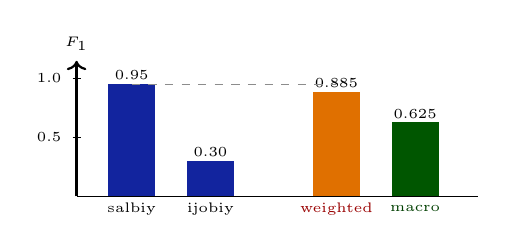
\begin{tikzpicture}[font=\tiny]
    \def\H{1.5}\def\bw{0.30}
    \draw[ax] (0,0) -- (0,\H+0.22) node[above]{$F_1$};
    \draw[thin] (-0.05,\H)--(0.05,\H);     \node[tlab,left] at (-0.07,\H){1.0};
    \draw[thin] (-0.05,0.5*\H)--(0.05,0.5*\H);\node[tlab,left] at (-0.07,0.5*\H){0.5};
    \draw[thin] (0,0)--(5.1,0);
    % har sinf F1
    \fill[cnublue] (0.7-\bw,0) rectangle (0.7+\bw,0.95*\H);
    \node[tlab] at (0.7,0.95*\H+0.11){0.95}; \node[tlab] at (0.7,-0.16){salbiy};
    \fill[cnublue] (1.7-\bw,0) rectangle (1.7+\bw,0.30*\H);
    \node[tlab] at (1.7,0.30*\H+0.11){0.30}; \node[tlab] at (1.7,-0.16){ijobiy};
    % weighted (aldaydi) -- ko'pchilik sinfga yopishadi
    \fill[orange!88!black] (3.3-\bw,0) rectangle (3.3+\bw,0.885*\H);
    \node[tlab] at (3.3,0.885*\H+0.11){0.885};
    \node[tlab,deepred] at (3.3,-0.16){weighted};
    % macro (to'g'riroq) -- ikki sinf o'rtasida
    \fill[deepgreen!75!black] (4.3-\bw,0) rectangle (4.3+\bw,0.625*\H);
    \node[tlab] at (4.3,0.625*\H+0.11){0.625};
    \node[tlab,deepgreen!55!black] at (4.3,-0.16){macro};
    % weighted ko'pchilik (salbiy) darajasiga yaqinligini ko'rsatadi
    \draw[helperln] (0.7,0.95*\H)--(3.3,0.95*\H);
  \end{tikzpicture}
  \end{center}
\end{frame}

% ================================================================
\section[Etika]{NLPda etika va adolat}
% ================================================================

% ----------------------------------------------------------------
% [F4] INTUITSIYA: model kimga zarar yetkazishi mumkin
% ----------------------------------------------------------------
\begin{frame}{Etika --- modelingiz kimga zarar yetkazishi mumkin?}
  \begin{columns}[T]
    \begin{column}{0.53\textwidth}
      \small
      \textbf{Vaziyat:}\\
      Kompaniya sentiment modeli
      barcha viloyatlar mijozlari
      sharhlarini baholaydi.\\[5pt]
      Train ma'lumotlari asosan Toshkent sharhlaridan yig'ilgan.\\[4pt]
      \begin{tcolorbox}[warnbox]
        \small
        Farg'ona shevasidagi so'zlar\\
        $\to$ lug'atda yo'q\\
        $\to$ ``salbiy'' standart bashorat\\
        $\to$ sistematik xato
      \end{tcolorbox}
    \end{column}
    \begin{column}{0.43\textwidth}
      \vspace{10pt}
      \begin{tcolorbox}[defbox,title=Agar hal qilinmasa]
        \small
        Hududiy mijozlar fikri to'g'ri baholanmaydi\\[3pt]
        Kompaniya mahsulotini
        faqat bir mintaqa uchun
        optimallashtiradi\\[3pt]
        \textbf{Adolat buziladi}
      \end{tcolorbox}
    \end{column}
  \end{columns}
\end{frame}

% ----------------------------------------------------------------
% [G4] UCH ETIKA MUAMMOSI
% ----------------------------------------------------------------
\begin{frame}{NLPda uch etika muammosi}
  \begin{tcolorbox}[warnbox,title=1.\ Bir tomonga og'gan (biased) ma'lumot]
    \footnotesize
    O'quv ma'lumotlari bir tomonga og'sa, model shu og'ishni takrorlaydi.\\
    Masalan, 95\% salbiy sharh bo'lsa, ijobiy o'zgarishlar ``ko'rinmay'' qoladi.
  \end{tcolorbox}
  \vspace{2pt}
  \begin{tcolorbox}[warnbox,title=2.\ Kam resursli til va dialekt]
    \footnotesize
    Dialekt yoki kam uchraydigan shakllar "out-of-vocabulary" (OOV) bo'lsa, model sistematik xato qiladi.\\
    Natijada, ayrim mintaqa foydalanuvchilari xizmat yoki kredit tizimida zarar ko'radi.
  \end{tcolorbox}
  \vspace{2pt}
  \begin{tcolorbox}[warnbox,title=3.\ Shaffoflik yetishmasligi]
    \footnotesize
    ``Arizangiz rad etildi'' degan natija sabab bilan izohlanmasa, apellyatsiya imkoni cheklanadi.\\
    Amaliy yechim: muhim so'zlar, ehtimollik, metrika va cheklovlarni hisobotda ko'rsatish.
  \end{tcolorbox}
\end{frame}

% ----------------------------------------------------------------
% [J4] MUHOKAMA: etika ssenariyi
% ----------------------------------------------------------------
\begin{frame}{Muhokama!}
  \begin{tcolorbox}[warnbox,title=Vaziyat (5 daqiqa)]
    \small
    Bank kreditiga ariza bergan shaxsning ijtimoiy tarmoq
    xabarlari sentiment modeli bilan baholanadi.\\[5pt]
    \begin{enumerate}
      \item Model o'zbek dialektlarini tanimaydi.
      \item  O'quv ma'lumoti: 90\% salbiy xabarlardan iborat.
      \item Natija faqat ``ijobiy/salbiy'' --- tushuntirish yo'q.
    \end{enumerate}
    \vspace{5pt}
    \textbf{Savollar:}\\[3pt]
    a)\; Bu tizimda yuqoridagi uch etika muammosining qaysilari mavjud?\\[3pt]
    b)\; Har bir muammo uchun bitta amaliy yechim taklif eting.\\[3pt]
    c)\; Modelni ``aniqroq'' qilish (accuracy ni oshirish) etika
         muammosini hal qiladimi?
  \end{tcolorbox}

\end{frame}

% ================================================================
\section[Xulosa]{Xulosa}
% ================================================================

% ----------------------------------------------------------------
% [M] O'ZBEK BURCHAGI: agglutinatsiya va tasniflash
% ----------------------------------------------------------------
\begin{frame}{O'zbek tili va tasniflash xususiyatlari}
  \begin{tcolorbox}[warnbox,title=Agglutinativ til va BoW muammosi]
    \small
    ``yaxshi'' $\neq$ ``yaxshiroq'' $\neq$ ``yaxshilik'' ---
    BoW da \textbf{uch alohida ustun}.\\
    Test to'plamidagi yangi shakl so'zlar lug'atga kirmasa, vektorlashtirishda yo'qolib ketadi.
    So'z lug'atda bor, lekin sinfda uchramagan bo'lsa, NB da
    $P(w\mid y){=}0$ xavfi paydo bo'ladi.
  \end{tcolorbox}
  \vspace{4pt}
  \begin{columns}[T]
    \begin{column}{0.49\textwidth}
      \begin{tcolorbox}[defbox,title=NB yondashuvi]
        \small
        NB yondashuvi: Laplace lug'atdagi, ammo ayrim sinfda uchramagan so'zlarni
        nol ehtimollikdan saqlaydi.\\
        Haqiqiy OOV uchun char n-gram yoki \texttt{<UNK>} kerak.
      \end{tcolorbox}
    \end{column}
    \begin{column}{0.49\textwidth}
      \begin{tcolorbox}[okbox,title=Yechim: preprocessing va n-gramlar]
        \small
        \texttt{preprocess()} ``yaxshiroq'', ``yaxshilik'' kabi shakllarni
        yagona asosga yaqinlashtiradi.\\
        Lug'at hajmi kamayadi, OOV xavfi pasayadi, lekin to'liq yo'qolmaydi.
      \end{tcolorbox}
    \end{column}
  \end{columns}
\end{frame}

% ----------------------------------------------------------------
% [N] SINTEZ: LR va NB taqqoslash jadvali
% ----------------------------------------------------------------
\begin{frame}{LR va NB: qaysi birini tanlash kerak?}
  \begin{center}
    \small
    \begin{tabular}{@{}lll@{}}
      \toprule
      Mezon & Logistik regressiya & Multinomial NB \\
      \midrule
      Tur & Diskriminativ & Generativ \\
      O'qitish & Iterativ (SGD) & Bir marta, tez \\
      Kichik korpus & regularizatsiya kerak & ko'pincha barqaror \\
      Katta korpus & \textcolor{deepgreen}{\textbf{Kuchli}} & Yetarlicha \\
      Korrelyatsiya & \textcolor{deepgreen}{\textbf{Bardoshli}} & Zaif (shartli mustaqillik muammosi)\\
      Interpretatsiya & $w_j$ koeffitsientlari & $P(w|y)$ \\
      O'zbek morfologiyasi & stemming / n-gram kerak & stemming / n-gram kerak \\
      Tengsiz sinf & \texttt{class\_weight}, threshold & \texttt{fit\_prior}, threshold \\
      \bottomrule
    \end{tabular}
  \end{center}
  \vspace{4pt}
  \small\textbf{Amaliy qoida:}
  kichik o'zbek korpus ($<$1000 namuna) $\to$ NB bilan baseline quring;
  keyin LR ni ham stratifikatsiyalangan validatsiyada sinab ko'ring.
\end{frame}

% ----------------------------------------------------------------
% [O] SEMINAL MAQOLA
% ----------------------------------------------------------------
\begin{frame}{O'qish uchun maqola: McCallum va Nigam (1998)}
  \begin{tcolorbox}[defbox,title=Maqola]
    \small
    McCallum, A., Nigam, K.\ (1998).\\
    \textit{A Comparison of Event Models for Naive Bayes
    Text Classification.}\\
    AAAI/ICML-98 Workshop on Learning for Text Categorization.
  \end{tcolorbox}
  \vspace{5pt}
  \small
  \textbf{Asosiy topilma:}
  Matn tasniflashda Multinomial NB ko'pincha Bernoulli NB dan ustun ---
  so'zlar chastotasini hisobga olish muhim.\\[4pt]
  Shu sababli bu kursda \texttt{CountVectorizer} + \texttt{MultinomialNB(alpha=1.0)} qo'llanilgan.\\[6pt]
  \begin{tcolorbox}[warnbox,title=Muhokama savoli (2-amaliyotgacha o'ylang)]
    \small
    Kichik o'zbek korpus (500 namuna) uchun LR yoki NB qaysi
    yaxshi ishlaydi?  Qanday eksperiment bilan aniqlaymiz?\\
    \textcolor{halfgray}{\footnotesize
      Maslahat: kross-validatsiya + macro $F_1$}
  \end{tcolorbox}
\end{frame}

% ----------------------------------------------------------------
% [P] MAQSADLAR BAJARILDI
% ----------------------------------------------------------------
\begin{frame}{Maqsadlar bajarildi}
  \begin{enumerate}\setlength{\itemsep}{9pt}
    \item \bajarildi  LR ---
          $\sigma(z)\to\ell_i\to L\to\partial L/\partial w_j$
          ni keltirib chiqardik.
    \item \bajarildi  NB posterior nisbati Laplace silliqlash bilan hisobladik.
    \item \bajarildi Confusion matrix dan
          $A{=}88\%$, $P{\approx}43\%$, $R{=}60\%$, $F_1{\approx}50\%$
          qurdik.
    \item \bajarildi Uch etika muammosi ---
          og'gan ma'lumot, kam resurs tili, shaffoflik yo'qligiga tanqidiy baho berdik.
  \end{enumerate}
\end{frame}

% ----------------------------------------------------------------
% [Q] KO'PRIK: P2 ga
% ----------------------------------------------------------------
\begin{frame}{Ertangi amaliyotda sentiment klassifikatori qurasiz}
  \begin{center}
    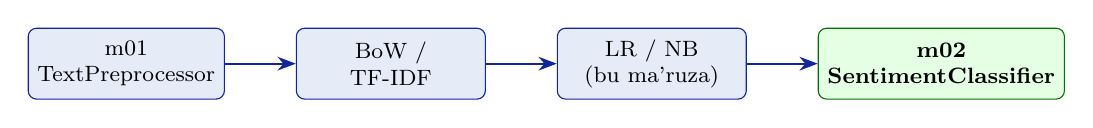
\begin{tikzpicture}[
      node distance=4mm and 9mm,
      box/.style={draw=cnublue,fill=cnubluebg,rounded corners=3pt,
                  minimum height=9mm,minimum width=24mm,
                  font=\footnotesize,align=center},
      goal/.style={draw=deepgreen,fill=green!10,rounded corners=3pt,
                   minimum height=9mm,minimum width=24mm,
                   font=\footnotesize\bfseries,align=center},
      arr/.style={-Stealth,cnublue,thick}
    ]
      \node[box]  (pre) {m01\\TextPreprocessor};
      \node[box,right=of pre] (vec) {BoW /\\TF-IDF};
      \node[box,right=of vec] (clf) {LR / NB\\(bu ma'ruza)};
      \node[goal,right=of clf](m02) {m02\\SentimentClassifier};
      \draw[arr] (pre)--(vec);
      \draw[arr] (vec)--(clf);
      \draw[arr] (clf)--(m02);
    \end{tikzpicture}
  \end{center}
  \vspace{4pt}
  \small 2-amaliyotda:
  \begin{itemize}
    \item \texttt{SentimentClassifier(m02)}:
          \texttt{fit()} / \texttt{predict()} / \texttt{predict\_proba()}
    \item LR va NB ni \texttt{macro $F_1$} bilan taqqoslash
    \item \texttt{confusion\_matrix} + \texttt{classification\_report} qurib ko'rasiz.
  \end{itemize}
  \vspace{4pt}
  \begin{tcolorbox}[warnbox,title=2-amaliyotning birinchi assert qiymati [28]-slayddan olinadi.]
    \footnotesize
    \texttt{assert abs(ratio - 3.375) < 0.01}\\
    \texttt{\# Ma'ruzaning [28]-slaydi bilan solishtiring}
  \end{tcolorbox}
\end{frame}

% ----------------------------------------------------------------
% [R] ADABIYOTLAR
% ----------------------------------------------------------------
\begin{frame}{Adabiyotlar}
  \small
  \begin{enumerate}\setlength{\itemsep}{5pt}
    \item McCallum, A., Nigam, K.\ (1998).
          \textit{A Comparison of Event Models for Naive Bayes
          Text Classification.} AAAI/ICML-98 Workshop.

    \item Jurafsky, D., Martin, J.H.\ (2024).
          \textit{Speech and Language Processing}, 3rd ed.\
          \S4 (Naive Bayes), \S5 (Logistic Regression),
          \S4.7 (Evaluation).
          \textcolor{halfgray}{\footnotesize
            \texttt{web.stanford.edu/\textasciitilde jurafsky/slp3/}}

    \item Pedregosa, F.\ et al.\ (2011).
          Scikit-learn: Machine Learning in Python.
          \textit{JMLR} 12, 2825--2830.
          \textcolor{halfgray}{\footnotesize
            \texttt{sklearn.naive\_bayes},
            \texttt{sklearn.linear\_model},
            \texttt{sklearn.metrics}}

    \item Mitchell, M.\ et al.\ (2019).
          Model Cards for Model Reporting.
          \textit{FAccT~'19.}
          \textcolor{halfgray}{\footnotesize
            Etika va shaffoflik standarti.}
  \end{enumerate}
\end{frame}

% ================================================================
\appendix
% ================================================================

% ----------------------------------------------------------------
% [S1] SIGMOID MATEMATIK XOSSALARI
% ----------------------------------------------------------------
\begin{frame}{Ilova S1: sigmoid xossalari va foydali farazlar}
  \small
  \begin{columns}[T]
    \begin{column}{0.55\textwidth}
      \textbf{Ta'rif:}\quad
      $\sigma(z)=\dfrac{1}{1+e^{-z}}$\\[6pt]
      \textbf{Hosila:}
      \[
        \sigma'(z)
        =\frac{e^{-z}}{(1+e^{-z})^2}
        =\sigma(z)\bigl(1-\sigma(z)\bigr)
      \]
      \textcolor{halfgray}{\footnotesize
        Isboti: $\tfrac{d}{dz}(1+e^{-z})^{-1}
        =(-1)(1+e^{-z})^{-2}(-e^{-z})$}\\[6pt]
      \textbf{Chegaralar:}\\[2pt]
      $\lim\limits_{z\to+\infty}\sigma(z)=1$;\quad
      $\lim\limits_{z\to-\infty}\sigma(z)=0$;\quad
      $\sigma(0)=0.5$
    \end{column}
    \begin{column}{0.44\textwidth}
      \centering
      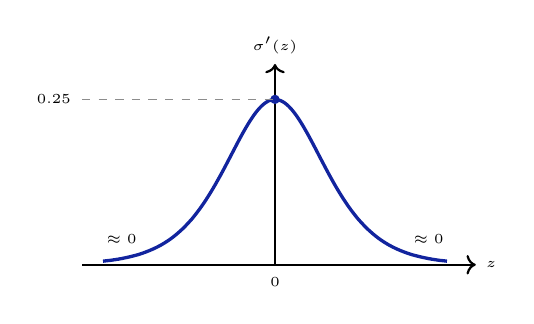
\begin{tikzpicture}[font=\tiny]
        \def\sx{0.42}\def\k{8.4}
        \draw[ax] (-2.45,0) -- (2.55,0) node[right]{$z$};
        \draw[ax] (0,0) -- (0,2.55) node[above]{$\sigma'(z)$};
        % qo'ng'iroqsimon egri: sigma'(z)=sigma(z)(1-sigma(z)), juft funksiya
        \draw[curveA,domain=-5.2:5.2,samples=90]
              plot ({\x*\sx},{exp(-abs(\x))/pow(1+exp(-abs(\x)),2)*\k});
        % maksimum 0.25 (z=0 da)
        \node[dotB] at (0,{0.25*\k}) {};
        \draw[helperln] (-2.45,{0.25*\k}) -- (0,{0.25*\k});
        \node[tlab,left] at (-2.47,{0.25*\k}) {0.25};
        \node[tlab,below] at (0,-0.04) {0};
        \node[tlab] at (1.95,0.32) {$\approx 0$};
        \node[tlab] at (-1.95,0.32) {$\approx 0$};
      \end{tikzpicture}\\[2pt]
      {\footnotesize\color{halfgray}Gradient $z{=}0$ (qaror chegarasi)
       da \emph{eng katta}; ishonchli bashoratda $\to 0$.}
    \end{column}
  \end{columns}
  \vspace{6pt}
  \textbf{Qo'lda hisob uchun farazlar:}\\[3pt]
  $e^{-0.5}\approx 0.607$;\quad
  $e^{0.5}\approx 1.649$;\quad
  $e^{1.5}\approx 4.48$;\quad
  $e^{-1.5}\approx 0.223$;\quad
  $e^{1}\approx 2.718$
\end{frame}

% ----------------------------------------------------------------
% [S2] BAYES TEOREMI CHIQARISHI
% ----------------------------------------------------------------
\begin{frame}{Ilova S2: Bayes teoremasini chiqarish}
  \small
  \textbf{Birgalik ehtimollik:}
  \[
    P(y)\cdot P(\mathbf{x}\mid y)
    = P(y,\mathbf{x})
    = P(\mathbf{x})\cdot P(y\mid\mathbf{x})
  \]
  \textbf{Shundan:}
  \[
    P(y\mid\mathbf{x})
    =\frac{P(\mathbf{x}\mid y)\,P(y)}{P(\mathbf{x})}
  \]
  \textbf{Klassifikatsiyada:}
  $P(\mathbf{x})$ barcha $y$ lar uchun bir xil
  $\Rightarrow$ proporsional yozish mumkin:
  \[
    P(y\mid\mathbf{x})\;\propto\; P(\mathbf{x}\mid y)\,P(y)
  \]
  Shu sababli NB da maxraj ($P(\mathbf{x})$) hisoblash shart emas ---
  faqat numeratorlarni taqqoslaymiz.
\end{frame}

% ----------------------------------------------------------------
% [S3] F-BETA FORMULASI
% ----------------------------------------------------------------
\begin{frame}{Ilova S3: $F_\beta$ formulasi}
  \small
  \begin{columns}[T]
    \begin{column}{0.55\textwidth}
      Agar Recall $R$ Precision $P$ dan muhimroq bo'lsa ($\beta>1$):
      \[
        F_\beta = \frac{(1+\beta^2)\,P\cdot R}{\beta^2\,P + R}
      \]
      \bunda{$\beta>1$: recallga ko'proq;\;
             $\beta<1$: precisionga ko'proq og'irlik}\\[5pt]
      \textbf{Misollar:}
      \begin{itemize}\setlength{\itemsep}{3pt}
        \item Tibbiy diagnoz: $\beta=2$ (FN qimmat)\\
              $F_2 = 5PR/(4P+R)$
        \item Spam filtri: $\beta=0.5$ (FP qimmat)\\
              $F_{0.5} = 1.25PR/(0.25P+R)$
        \item Standart sentiment: $\beta=1 \Rightarrow F_1 = 2PR/(P+R)$
      \end{itemize}
    \end{column}
    \begin{column}{0.44\textwidth}
      \centering
      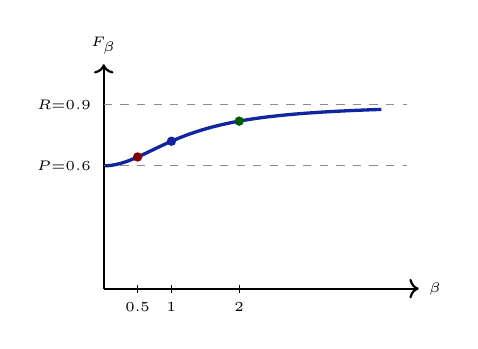
\begin{tikzpicture}[font=\tiny]
        \def\sx{0.86}\def\H{2.6}
        \draw[ax] (0,0) -- (4.0,0) node[right]{$\beta$};
        \draw[ax] (0,0) -- (0,\H+0.25) node[above]{$F_\beta$};
        % P va R asimptotalari
        \draw[helperln] (0,{0.6*\H}) -- (3.85,{0.6*\H});
        \node[tlab,left] at (-0.04,{0.6*\H}) {$P{=}0.6$};
        \draw[helperln] (0,{0.9*\H}) -- (3.85,{0.9*\H});
        \node[tlab,left] at (-0.04,{0.9*\H}) {$R{=}0.9$};
        % F_beta egri chizig'i (P=0.6, R=0.9)
        \draw[curveA,domain=0.02:4.1,samples=110]
              plot ({\x*\sx},{(1+\x*\x)*0.6*0.9/(\x*\x*0.6+0.9)*\H});
        % belgilangan beta nuqtalari
        \draw[thin] (0.5*\sx,-0.05)--(0.5*\sx,0.05);
        \draw[thin] (1*\sx,-0.05)--(1*\sx,0.05);
        \draw[thin] (2*\sx,-0.05)--(2*\sx,0.05);
        \node[tlab,below] at (0.5*\sx,-0.05){0.5};
        \node[tlab,below] at (1*\sx,-0.05){1};
        \node[tlab,below] at (2*\sx,-0.05){2};
        \node[dotR] at (0.5*\sx,{0.643*\H}){};
        \node[dotB] at (1*\sx,{0.72*\H}){};
        \node[dotG] at (2*\sx,{0.818*\H}){};
      \end{tikzpicture}\\[2pt]
      {\footnotesize\color{halfgray}$\beta$ kichik $\to F\!\approx\!P$;\;
       $\beta$ katta $\to F\!\approx\!R$.}
    \end{column}
  \end{columns}
\end{frame}

\end{document}
